% !TEX encoding = UTF-8 Unicode

\documentclass[aspectratio=169]{beamer}
\usepackage[utf8]{inputenc}

%% BIB
\usepackage[
  style=authoryear,
  backend=biber,
  url=false,
  maxcitenames=2,
  uniquename=false,
  uniquelist=false
]{biblatex}
%\addbibresource{?.bib}

%% GRAPHICS

\usepackage{graphicx}
\graphicspath{{images/},{figures/}}
\usepackage{tikz}

%% COLORS
\definecolor{UWRed}{HTML}{C5050C}
\definecolor{TintedBG}{HTML}{EEEEFF}
%\definecolor{StrongBlue}{HTML}{3F8FD2}
%\definecolor{StrongGreen}{HTML}{36C88E}
%\definecolor{StrongRed}{HTML}{9B0000}
%\definecolor{MyC}{HTML}{009999}
%\definecolor{MyM}{HTML}{990099}
%\definecolor{MyY}{HTML}{999900}
%\definecolor{MyR}{HTML}{990000}
%\definecolor{MyG}{HTML}{009900}
%\definecolor{MyB}{HTML}{000099}
%\definecolor{ActionRed}{HTML}{990000}

%% SLIDE COLOR SETTINGS
\setbeamercolor{structure}{fg=UWRed}
\setbeamercolor{title page}{fg=white}
\setbeamercolor{title}{fg=white}

%% RM NAV SYMBOLS
\setbeamertemplate{navigation symbols}{}

%% FONTS
\setbeamerfont{title}{size=\huge\bfseries}

%% DRAWING
%\usetikzlibrary{}

\def\firstcircle{(90:0.3cm) circle (0.6cm)}
\def\secondcircle{(210:0.3cm) circle (0.6cm)}
\def\thirdcircle{(330:0.3cm) circle (0.6cm)}

%% LOGO on slides
\logo{\begin{tikzpicture}[overlay]
  \node[anchor=north east,inner sep=0] at (0,86mm) {
\includegraphics[height=10mm]{SMPH_color-flush.pdf}};
\end{tikzpicture}}

%% CONTENT BEGINS

\title{Anchors (and other) High-Precision Model-Agnostic Explanations}
\subtitle{AIRG Presentation}
\author{Yuriy Sverchkov}
\institute{University of Wisconsin--Madison}
\date{October 31, 2018}

\begin{document}

  {
    \setbeamertemplate{background canvas}{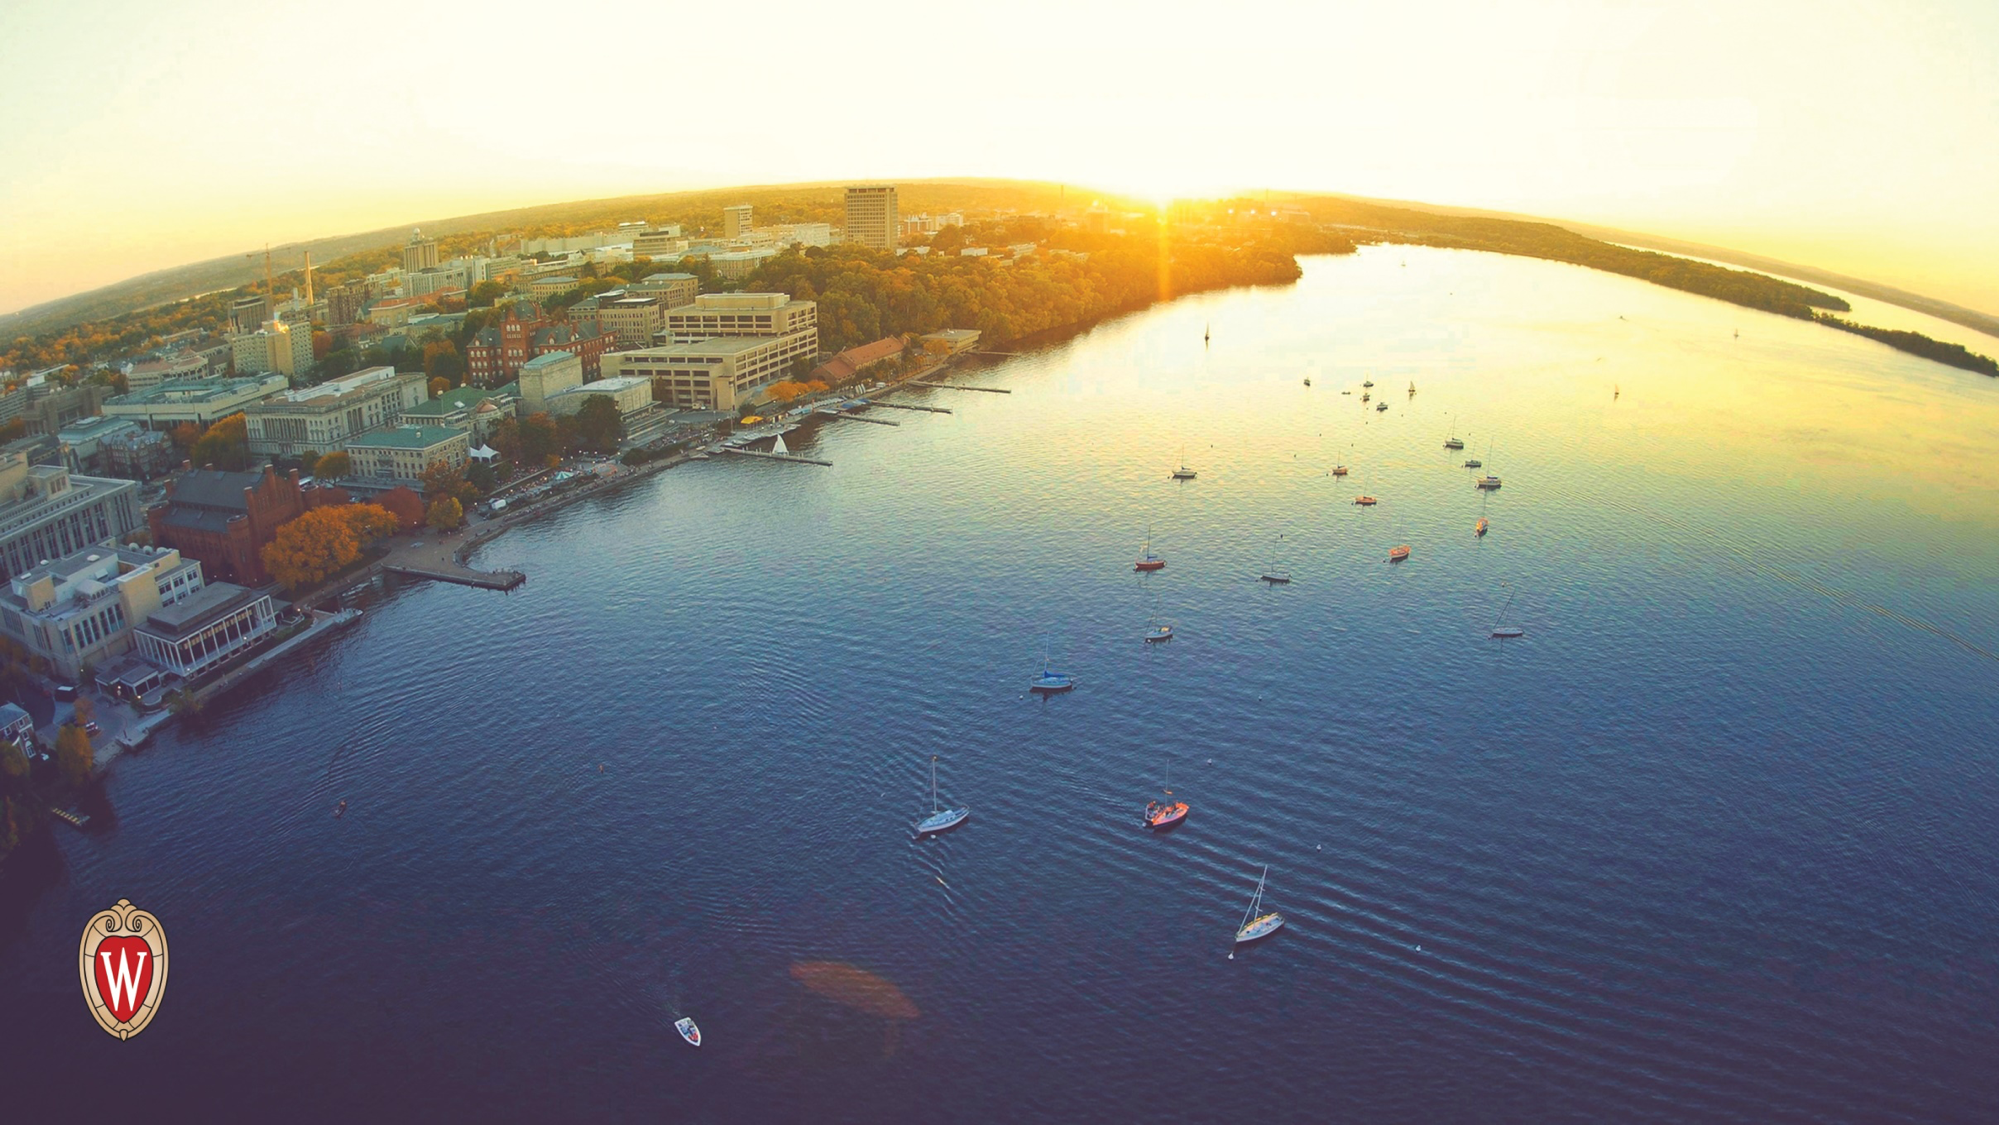
\includegraphics[width=\paperwidth]{UW-lake.png}}
    \begin{frame}[plain]
      \vskip4cm
      \titlepage
    \end{frame}
  }

%%% FRAMEBREAK %%%

% Motivation:
%  (many good ml systems are black box)
%  "chat vignette": what dis? cat! why? math! *confused* ; better explanation
%
%  (there is a need from)
%  policymakers/legal: GDPR (find the ref)
%  high-risk decision-makers: (doctors/critical systems/self-driving)
%  explanations build trust (find a ref?)

\begin{frame}{\textbf{Why} should we \textbf{explain} our models?}

\begin{itemize}[<+->]
	\item Many of the best-performing machine learning models are not (easily) \textbf{interpretable} (by non-ML experts)
	\item Users need explanations:
	\begin{itemize}
		\item when using models for medical decisions
		\item when using models for policymaking
		\item in other high-risk decision support
		\item for legal reasons
	\end{itemize}
\end{itemize}
\pause

\textbf{GDPR Article 13(2f)} [The data subject shall be informed of] the existence of automated decision-making [... and provided] meaningful information about the logic involved

\begin{itemize}[<+->]
	\item Explanations build trust in a good model
	\item Explanations can help troubleshoot a bad model
\end{itemize}
\end{frame}

%%% FRAMEBREAK %%%

\begin{frame}
\vfill

\centering
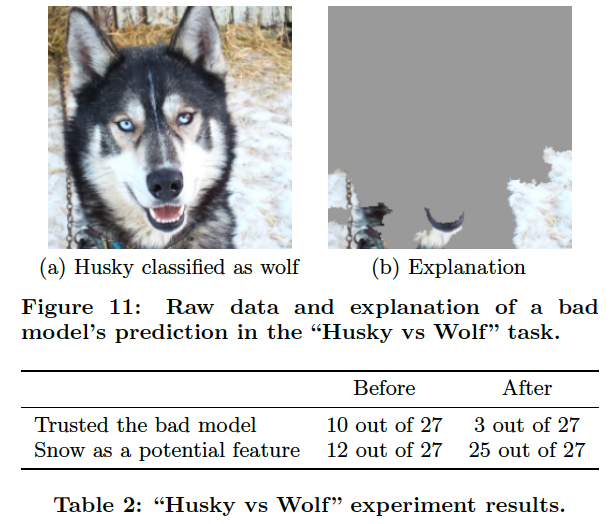
\includegraphics[width=6cm]{LIME-wolf.png}

\vfill

\raggedleft
\scriptsize
Ribiero, Singh, and Guestrin, SIGKDD 2016
\end{frame}

%%% FRAMEBREAK %%%

\begin{frame}{Interpretable models}
\begin{columns}
	\column[T]{0.45\textwidth}
	\begin{center}\bf Interpretable \end{center}
	\begin{itemize}
		\item Generalized linear models
		\item[] $y = g^{-1}( X\beta )$
		\item[] %TODO! make illustration explaining how to interpret linear model
		\item Rules and decision trees
		%\item [] example?
	\end{itemize}
	
	\column[T]{0.45\textwidth}
	\begin{center}\textbf{Uninterpretable} or "black box"\end{center}
	% image refs, for ai box: fico.com
	% for steampunk box: https://www.lindacohendesigns.com
	
	$y = \sigma( W^1 \sigma( W^2 \sigma( W^3 X ) ) )$
	
\end{columns}
\end{frame}
  
%%% FRAMEBREAK %%%

\begin{frame}{Explanation}
\begin{itemize}[<+->]
	\item Uninterpretable $\rightarrow$ Interpretable
	\item TREPAN (Craven and Shavlik, NIPS 1996)
	\item[] Decision tree
	\item LIME (Ribiero, Singh, and Guestrin, SIGKDD 2016)
	\item[] (locally) Linear model
	\item Anchors () % TODO
	\item[] Conjunctive rules
\end{itemize}

\end{frame}

%%% FRAMEBREAK %%%

\begin{frame}{TREPAN} % TODO
\begin{columns}
	\column{0.5\textwidth}
	\begin{itemize}[<+->]
		\item Learns a decision tree from a neural network (NN)
		\item A big challenge to learning decision trees from data is that the amount of relevant samples decreases as the tree gets deeper
		\item TREPAN uses the NN for an oracle to evaluate splits, eliminating this issue
		\item Decision nodes ($n$) to expand are prioritized by
		\item[] $\mathit{reach}( n ) \times (1 - \mathit{fidelity}(n) )$
	\end{itemize}
	\column{6cm}
	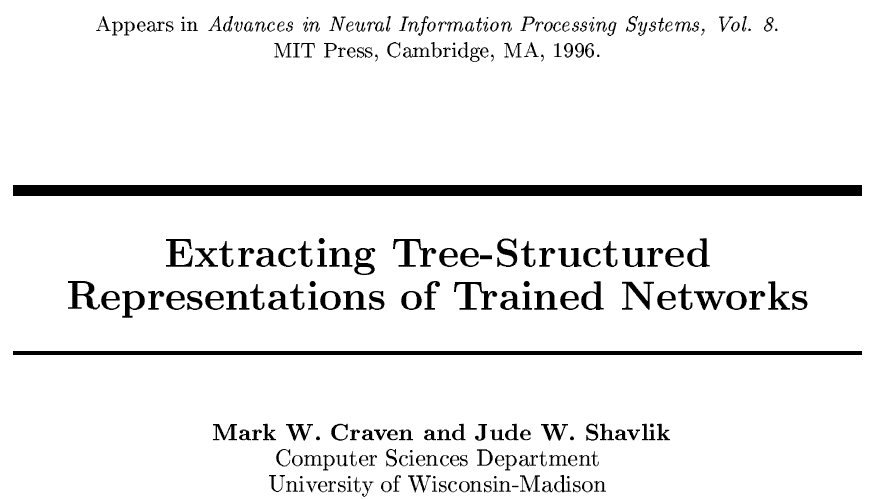
\includegraphics[width=6cm]{trepan-title.png}
\end{columns}
\end{frame}

%%% FRAMEBREAK %%%

\begin{frame}{LIME}
\begin{columns}
	\column{0.47\textwidth} \centering
	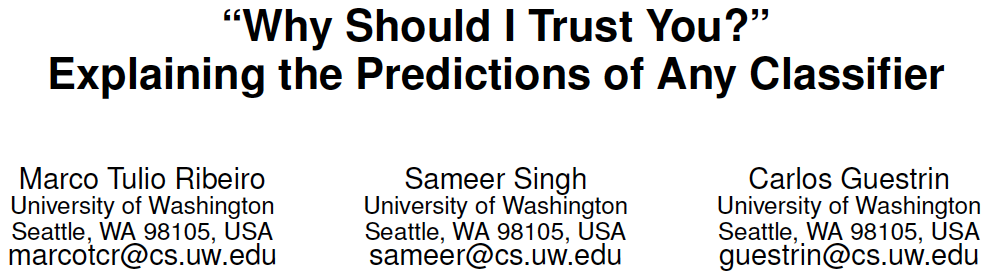
\includegraphics[width=6cm]{LIME-title.png}
	
	{\color{UWRed}
	\[
	\arg \min_g \underbrace{ \mathcal L ( f, g, \pi_x ) }_{\text{fidelity loss around }x} + \underbrace{ \Omega( g ) }_\text{complexity}
	\]}
	
	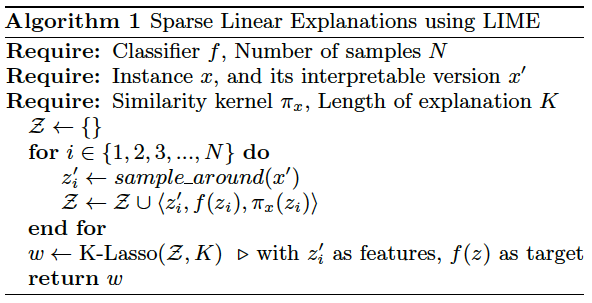
\includegraphics[width=6cm]{LIME-alg.png}
	\column{0.47\textwidth} \centering
	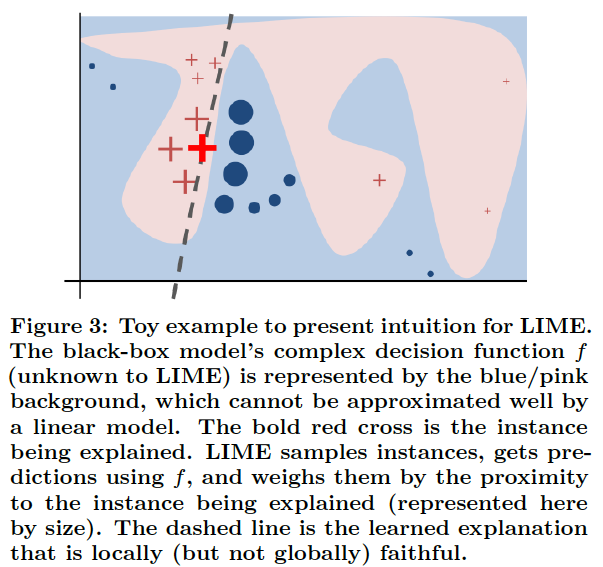
\includegraphics[width=6cm]{LIME-intuition.png}
\end{columns}
\end{frame}

%%% FRAMEBREAK %%%

\begin{frame}{LIME applied to images}
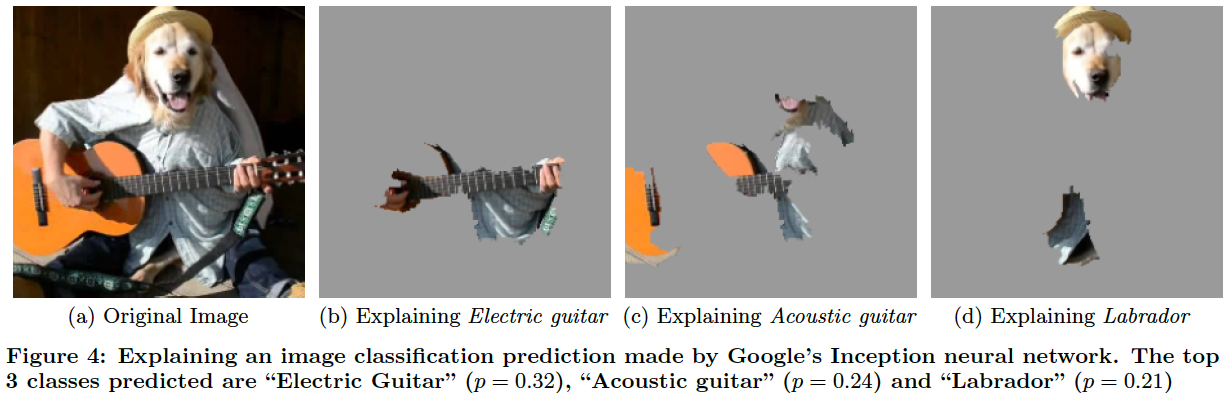
\includegraphics[width=\textwidth]{LIME-image.png}
\end{frame}

%%% FRAMEBREAK %%%



%%% FRAMEBREAK %%%

\begin{frame}{Anchor: formal definition}
  Given a black-box model $f : X \rightarrow Y$
  
  $X$ is the space of instances, $Y$ is the space of model outputs.
  
  $A : X \rightarrow \{0,1\}$ is an anchor iff
  
  $\underbrace{\mathbb{E}_{\mathcal D (z | A)} \left[ \mathbf{1}_{f(x)=f(z)} \right] }_{\mathrm{Prec}(A)} \geq \tau$ when $A(x) = 1$
  
  That is, $A$ is a rule that holds for our sample $x$ and, for any $z$ in the data distribution for which $A$ holds, the output is (probably) the same as for $x$.
\end{frame}

% TODO:

%  Sidebar about the difference between a "classical statistician" and a "machine learning expert" when using logistic regression
%
% Go over main paper in detail:
%  What's an "Anchor" -- examples and tasks
%    text classification
%    structured prediction
%    tabular classification
%    image classification
%    visual question answering
%  What's an Anchor mathematically (formula) -DONE (sort of)
%
%  How to find anchors: greedy build up
%   candidates are built up by adding feature predicates to candidate anchors
%   candidate precision is sampled from a distrinution
%   uses KL-LUCB (look up? briefly describe? Kaufmann and Kalyanakrishnan 2013)
%   select rules for best mean (A) and highest upperbound (A')
%
%  Comparison to LIME (briefly summarize LIME)
%
%  Experiments with users

%%% FRAMEBREAK %%%

\begin{frame}{a frame}
with text
\end{frame}

\end{document}